\PassOptionsToPackage{unicode=true}{hyperref} % options for packages loaded elsewhere
\PassOptionsToPackage{hyphens}{url}
%
\documentclass[british,,man,floatsintext]{apa6}
\usepackage{lmodern}
\usepackage{amssymb,amsmath}
\usepackage{ifxetex,ifluatex}
\usepackage{fixltx2e} % provides \textsubscript
\ifnum 0\ifxetex 1\fi\ifluatex 1\fi=0 % if pdftex
  \usepackage[T1]{fontenc}
  \usepackage[utf8]{inputenc}
  \usepackage{textcomp} % provides euro and other symbols
\else % if luatex or xelatex
  \usepackage{unicode-math}
  \defaultfontfeatures{Ligatures=TeX,Scale=MatchLowercase}
\fi
% use upquote if available, for straight quotes in verbatim environments
\IfFileExists{upquote.sty}{\usepackage{upquote}}{}
% use microtype if available
\IfFileExists{microtype.sty}{%
\usepackage[]{microtype}
\UseMicrotypeSet[protrusion]{basicmath} % disable protrusion for tt fonts
}{}
\IfFileExists{parskip.sty}{%
\usepackage{parskip}
}{% else
\setlength{\parindent}{0pt}
\setlength{\parskip}{6pt plus 2pt minus 1pt}
}
\usepackage{hyperref}
\hypersetup{
            pdftitle={Incentives for a safe publication option from a risk sensitivity perspective},
            pdfauthor={Anne M. Scheel1, Leo Tiokhin1, \& Daniël Lakens1},
            pdfkeywords={Publication bias, Registered Reports, hypothesis testing},
            pdfborder={0 0 0},
            breaklinks=true}
\urlstyle{same}  % don't use monospace font for urls
\usepackage{graphicx,grffile}
\makeatletter
\def\maxwidth{\ifdim\Gin@nat@width>\linewidth\linewidth\else\Gin@nat@width\fi}
\def\maxheight{\ifdim\Gin@nat@height>\textheight\textheight\else\Gin@nat@height\fi}
\makeatother
% Scale images if necessary, so that they will not overflow the page
% margins by default, and it is still possible to overwrite the defaults
% using explicit options in \includegraphics[width, height, ...]{}
\setkeys{Gin}{width=\maxwidth,height=\maxheight,keepaspectratio}
\setlength{\emergencystretch}{3em}  % prevent overfull lines
\providecommand{\tightlist}{%
  \setlength{\itemsep}{0pt}\setlength{\parskip}{0pt}}
\setcounter{secnumdepth}{0}

% set default figure placement to htbp
\makeatletter
\def\fps@figure{htbp}
\makeatother

% Manuscript styling
\usepackage{upgreek}
\captionsetup{font=singlespacing,justification=justified}

% Table formatting
\usepackage{longtable}
\usepackage{lscape}
% \usepackage[counterclockwise]{rotating}   % Landscape page setup for large tables
\usepackage{multirow}		% Table styling
\usepackage{tabularx}		% Control Column width
\usepackage[flushleft]{threeparttable}	% Allows for three part tables with a specified notes section
\usepackage{threeparttablex}            % Lets threeparttable work with longtable

% Create new environments so endfloat can handle them
% \newenvironment{ltable}
%   {\begin{landscape}\begin{center}\begin{threeparttable}}
%   {\end{threeparttable}\end{center}\end{landscape}}
\newenvironment{lltable}{\begin{landscape}\begin{center}\begin{ThreePartTable}}{\end{ThreePartTable}\end{center}\end{landscape}}

% Enables adjusting longtable caption width to table width
% Solution found at http://golatex.de/longtable-mit-caption-so-breit-wie-die-tabelle-t15767.html
\makeatletter
\newcommand\LastLTentrywidth{1em}
\newlength\longtablewidth
\setlength{\longtablewidth}{1in}
\newcommand{\getlongtablewidth}{\begingroup \ifcsname LT@\roman{LT@tables}\endcsname \global\longtablewidth=0pt \renewcommand{\LT@entry}[2]{\global\advance\longtablewidth by ##2\relax\gdef\LastLTentrywidth{##2}}\@nameuse{LT@\roman{LT@tables}} \fi \endgroup}

% \setlength{\parindent}{0.5in}
% \setlength{\parskip}{0pt plus 0pt minus 0pt}

% Overwrite redefinition of paragraph and subparagraph by the default LaTeX template
% See https://github.com/crsh/papaja/issues/292
\makeatletter
\renewcommand{\paragraph}{\@startsection{paragraph}{4}{\parindent}%
  {0\baselineskip \@plus 0.2ex \@minus 0.2ex}%
  {-1em}%
  {\normalfont\normalsize\bfseries\itshape\typesectitle}}

\renewcommand{\subparagraph}[1]{\@startsection{subparagraph}{5}{1em}%
  {0\baselineskip \@plus 0.2ex \@minus 0.2ex}%
  {-\z@\relax}%
  {\normalfont\normalsize\itshape\hspace{\parindent}{#1}\textit{\addperi}}{\relax}}
\makeatother

% \usepackage{etoolbox}
\makeatletter
\patchcmd{\HyOrg@maketitle}
  {\section{\normalfont\normalsize\abstractname}}
  {\section*{\normalfont\normalsize\abstractname}}
  {}{\typeout{Failed to patch abstract.}}
\patchcmd{\HyOrg@maketitle}
  {\section{\protect\normalfont{\@title}}}
  {\section*{\protect\normalfont{\@title}}}
  {}{\typeout{Failed to patch title.}}
\makeatother

\usepackage{xpatch}
\makeatletter
\xapptocmd\appendix
  {\xapptocmd\section
    {\addcontentsline{toc}{section}{\appendixname\ifoneappendix\else~\theappendix\fi\\: #1}}
    {}{\InnerPatchFailed}%
  }
{}{\PatchFailed}
\keywords{Publication bias, Registered Reports, hypothesis testing}
\usepackage{csquotes}
\usepackage{float}
\usepackage{framed}
\usepackage{caption}
\usepackage{setspace}
\usepackage{amsmath}
\captionsetup[figure]{font={stretch=1, small}, skip=10pt}
\captionsetup[textbox]{name=Box,labelsep=period,labelfont=it}
\newfloat{textbox}{thp}{lop}
\floatname{textbox}{Box}
\usepackage[most]{tcolorbox}
\definecolor{electricviolet}{rgb}{0.56, 0.0, 1.0}
\ifnum 0\ifxetex 1\fi\ifluatex 1\fi=0 % if pdftex
  \usepackage[shorthands=off,main=british]{babel}
\else
  % load polyglossia as late as possible as it *could* call bidi if RTL lang (e.g. Hebrew or Arabic)
  \usepackage{polyglossia}
  \setmainlanguage[variant=british]{english}
\fi

\title{Incentives for a safe publication option from a risk sensitivity perspective}
\author{Anne M. Scheel\textsuperscript{1}, Leo Tiokhin\textsuperscript{1}, \& Daniël Lakens\textsuperscript{1}}
\date{}


\shorttitle{Risk sensitivity in academic publishing}

\authornote{

Correspondence concerning this article should be addressed to Anne M. Scheel, Den Dolech 1, Atlas 9.417, 5600 MB, Eindhoven, The Netherlands. E-mail: \href{mailto:a.m.scheel@tue.nl}{\nolinkurl{a.m.scheel@tue.nl}}

}

\affiliation{\vspace{0.5cm}\textsuperscript{1} Eindhoven University of Technology}

\abstract{%
xxx Abstract xxx
}



\begin{document}
\maketitle

\begin{itemize}
\tightlist
\item
  publication bias \& QRPs
\item
  Registered Reports

  \begin{itemize}
  \tightlist
  \item
    what they are
  \item
    how they protect against bias
  \item
    evidence
  \end{itemize}
\item
  however, little data is available about the demographics of RR authors and characteristics of the research questions studied in RRs.
\end{itemize}

Being a powerful bias-prevention tool that is increasingly popular, it is important to develop a better understanding of when, where, and by whom Registered Reports are most likely to be used.
First, such knowledge can help identify research areas in which the format is unlikely to gain traction by itself and anticipate the need for further intervention (e.g., via policy) when there is a demand for unbiased results.
Second, understanding when researchers' choice between Registered Reports and the standard publication route is likely to be influenced by factors that also influence the eventual results (e.g., the prior probability of the studied hypotheses) is important for meta-scientific studies that compare published studies in both formats and must take such confounds into account (e.g., {\textbf{???}}).
As a final, perhaps less urgent motivation for such research, \ldots{} RISK OF DEVALUATION LIKE JOURNALS OF NEGATIVE RESULTS
The goal of this chapter is to shed light on these questions by studying the potential impact of a key feature of Registered Reports: results-independent publication guarantee as an incentive for authors.

\hypertarget{registered-reports-as-a-low-risk-publication-option}{%
\subsection{Registered Reports as a low-risk publication option}\label{registered-reports-as-a-low-risk-publication-option}}

In addition to protecting against publication bias and QRPs, Registered Reports are designed to \enquote{serve the interests of individual scientists} (p.~12, {\textbf{???}}) by providing a publication guarantee irrespective of the study results.
As such, Registered Reports make use of existing incentive structures in academia and do not rely on changes in norms or policy (in contrast to other reforms such as preregistration () or data sharing ()).

Amount and impact of peer-reviewed publications is a central currency for academic researchers {[}add some evidence{]}. In the standard publication model, researchers face uncertainty about whether and where they will be able to publish the results of their study. Translated into currency terms, the payoff a researcher receives for conducting a study can vary extremely: from near zero when the resulting manuscript is rejected by all peer-reviewed journals the author submits to --- or when the author file-drawers the study because the chances of successful publication appear too low to justify the costs of submission and peer review --- to an extremely high, perhaps career-making amount when a manuscript is published in a high-impact journal like Nature or Science.

The basic argument is that partly because of publication bias, publication success in the normal system is highly volatile and dependent on the one factor that is supposed to be outside of researchers' control\(\,\)---\(\,\)the results\(\,\)---\(\,\), putting especially early-career researchers under excessive stress and tempting them to hype, spin, or even fabricate their data.
Because publication is results-independent in Registered Reports and authors receive an in-principle acceptance before investing in data collection or analysis, the format is a relatively safe, stress-free alternative.
As Registered-Reports inventor Chris Chambers put it in a recent talk (September 2021):

\begin{quote}
And the second main benefit, the one that really is the main big one, the big draw, is that as a researcher you can get your paper accepted before you even start your research and regardless of how the results turn out in the end. So no more playing the \emph{p}-value lottery, gambling on certain results going a certain way, otherwise you won't have your PhD or you won't get your next fellowship or your next grant\(\,\)---\(\,\)takes all of that pointless, and I think quite foolish, gambling out of the equation completely. (from minute 17:27)
\end{quote}

But would researchers ever choose the gamble over the safe publication?
Unless the net benefit of a Registered Report is always at least as valuable as the best possible outcome that could be achieved through the standard publication route, the answer is \enquote{probably yes}.
Authors deciding between Registered Reports and the standard publication route face the choice between a payoff with low variability (a relatively safe publication in the journal the Stage-1 protocol was submitted to) and a payoff with high variability (anywhere between no publication and a high-impact publication, or even several publications if the project yields enough \enquote{fodder}).
Situations like these are commonly termed \emph{decision-making under risk}, where \enquote{risk} is defined as \enquote{unpredictable variation in the outcome of a behavior, with consequences for an organism's fitness or utility} (Winterhalder, Lu, \& Tucker, 1999, p. 302).
When organisms are sensitive not only to the mean outcomes of different options but also to their variance, they are called \enquote{risk sensitive}.

\begin{itemize}
\tightlist
\item
  Humans are risk-sensitive, therefore researchers should be too
  Like virtually all other organisms, humans are sensitive to risk but do not universally try to minimise (risk aversion) or maximise (risk proneness) it.
\end{itemize}

A large body of literature shows that humans

\begin{itemize}
\item
  RST is an explanatory theory for these situations
  Risk-Sensitivity Theory, a normative theory developed in behavioural ecology to explain foraging behaviour of animals
  Risk-Sensitivity Theory was originally developed to determine the optimal food-acquisition strategy for animals faced with a choice between a relatively safe (low-variance) food source and a risky (high-variance) source that sometimes yields large payoffs and sometimes small payoffs (or none at all).
  Despite this initial narrow scope, Risk-Sensitivity Theory has been successfully applied to humans as well as several non-human animal species (Kacelnik \& Bateson, 1996, 1997; Mishra, 2014; {[}add more refs{]}).
\item
  What does the argument entail?

  \begin{itemize}
  \tightlist
  \item
    RRs are \enquote{safer} than non-RRs --\textgreater{} less variance, less risk
  \item
    (safer = better)
  \item
    However, the argument that RRs are always more attractive for authors only holds if a) RRs are always worth at least as much as a normal publication or b) authors are always risk averse
  \end{itemize}
\item
  Enter Risk Sensitivity Theory

  \begin{itemize}
  \tightlist
  \item
    background
  \item
    basics
  \item
    comparison to utility theory and prospect theory
  \end{itemize}
\item
  RRs through an RST lens
\end{itemize}

\hypertarget{goals}{%
\subsection{Goals}\label{goals}}

\begin{itemize}
\tightlist
\item
  Understand under which circumstances RRs are unlikely to be viable
\item
  Understand how authors' strategic risk-sensitive decision-making may affect what is studied in RRs/the differe
\end{itemize}

This chapter explores how properties of academic careers and academic incentive structures that are relevant to risk sensitivity may affect the strategies of researchers choosing between Registered Reports and the standard publication format.
The research goal is to understand in which circumstances Registered Reports should be particularly attractive, particularly unattractive, or particularly prone to highly selective use, which would make their results difficult to compare to the normal literature.
The following section outlines central concepts of Risk-Sensitivity Theory, relates them to characteristics of academic careers, and describes a simulation model in which their effects on researchers' risk-sensitive publication decisions are examined.

\hypertarget{conceptual-application-of-risk-sensitivity-theory-to-researchers-publication-decisions}{%
\section{Conceptual application of Risk-Sensitivity Theory to researchers' publication decisions}\label{conceptual-application-of-risk-sensitivity-theory-to-researchers-publication-decisions}}

The following section describes general factors that affect the role of risk for individual's fitness and connects these factors to relevent elements of academic careers. \textbf{NEEDS REPHRASING B/C PREVIOUS PARAGRAPH WAS CHANGED}
In this context, Risk-Sensitivity Theory's focus on reproductive fitness as the central outcome may be seen as problematic.
But although researchers do not forage, grow, reproduce, and die in the \emph{biological} sense (except in their role as human beings in general, of course), they undoubtedly are concerned with factors that influence their survival and the propagation of their traits in an \emph{academic} sense.
In applying Risk-Sensitivity Theory to researchers' publishing behaviour, we will therefore use a general notion of career success as the central outcome variable in place of reproductive fitness.
This decision does not imply that career success is the sole proximal motivation for researchers' behaviour in practice, just as evolutionary theory does not imply that reproductive success is the sole proximal motivation for every person's everyday decisions.
\textbf{NEEDS WORK:}
However, being a product of evolution, human decision making has been shown to be risk sensitive in many domains.
significant competition for tenured positions in many academic disciplines inevitably creates a selection pressure for behaviours that further researchers' career success (Smaldino \& McElreath, 2016).

\hypertarget{non-linear-fitness-functions}{%
\paragraph{Non-linear fitness functions}\label{non-linear-fitness-functions}}

The first and perhaps most important factor leading individuals to be risk sensitive are non-linear relationships between the outcomes of an individual's behaviour (e.g., harvested food items, publications) and its reproductive success (fitness).
Consider two options, \(O_{safe}\) and \(O_{risky}\).
\(O_{safe}\) always gives the same payoff \(b_{safe}\), whereas \(O_{risky}\) gives either a low payoff \(b_-\) or a high payoff \(b_+\), each with probability \(\frac{1}{2}\).
When \(b_{safe} = \frac{(b_- + b_+)}{2}\), \(O_{safe}\) and \(O_{risky}\) have the same expected payoff.
However, we would only expect an individual to be indifferent between the two options if the consequences of their payoffs for the individual's fitness are linear.
When the function relating payoffs to utility is instead convex or concave (yielding increasing or diminishing returns, respectively), the expected utility of \(O_{safe}\) and \(O_{risky}\) will differ and shift the individual's preference towards risk proneness or risk aversion.
An illustration of this example is shown in Figure~\ref{fig:fitnessplot}:
While the payoffs \(b_-\), \(b_{safe}\), and \(b_+\) are equidistant on the x-axis, \(b_{safe}\) is associated with greater fitness than the average of \(b_-\) and \(b_+\) when the fitness function is concave and with less fitness when the fitness function is convex.



\begin{figure}
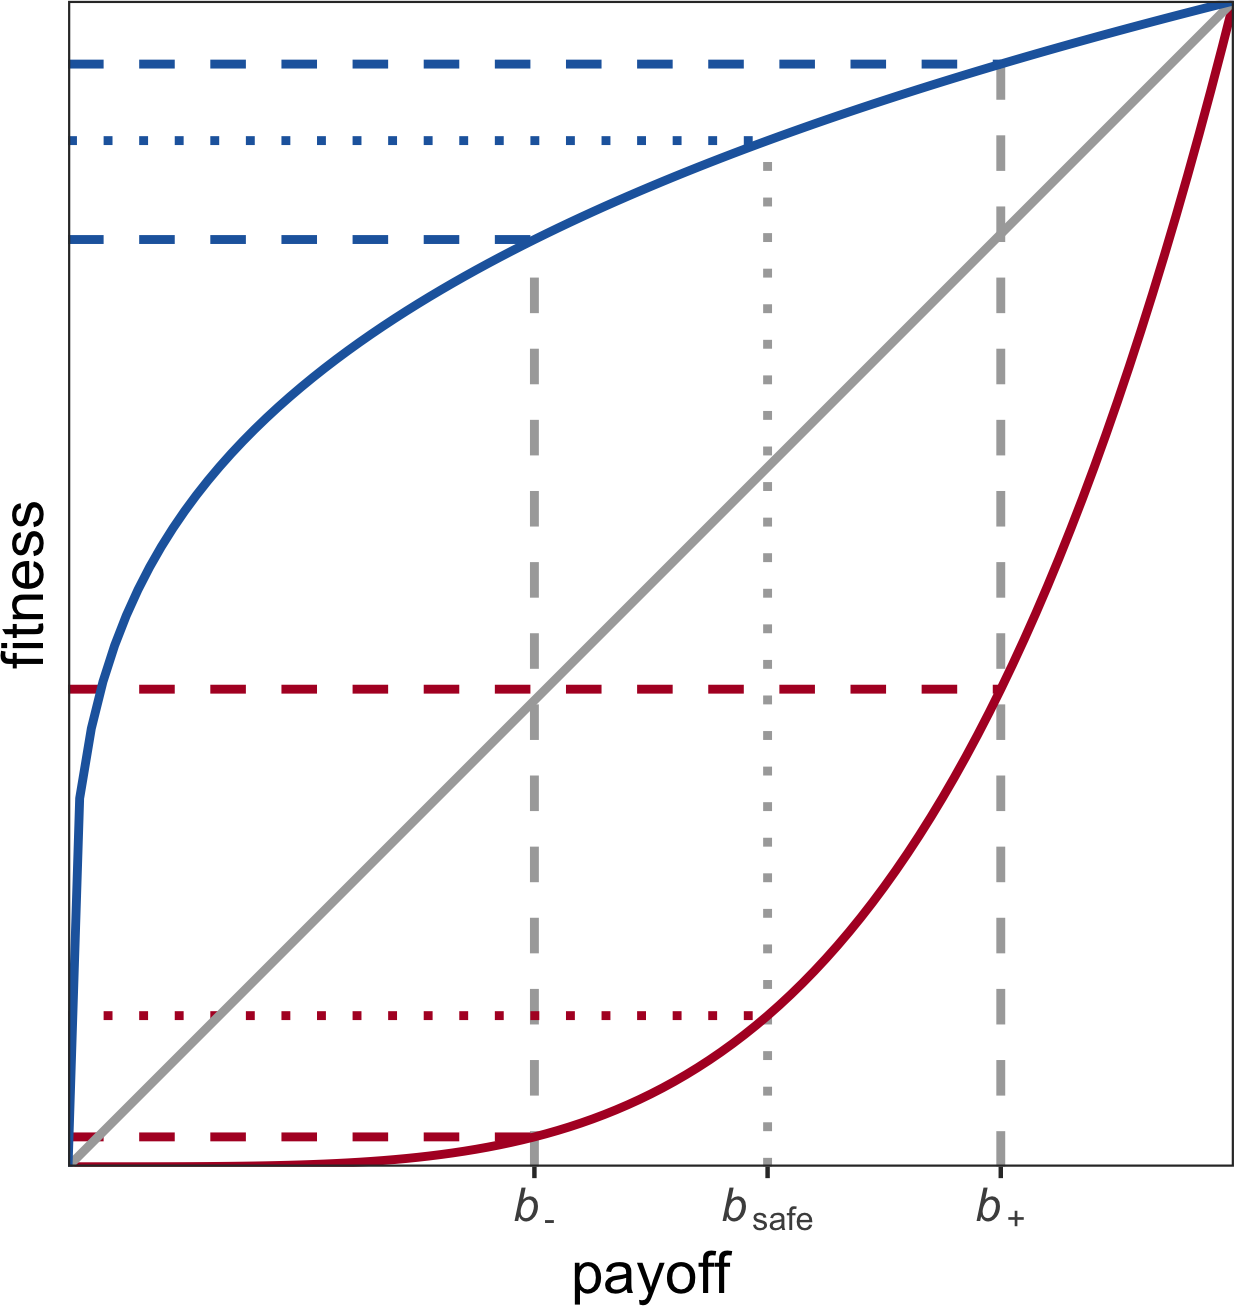
\includegraphics[width=0.5\linewidth]{rr-risk-sensitivity_files/figure-latex/fitnessplot-1} \caption{Consequences of non-linear fitness functions. Payoffs \(b_-\), \(b_{safe}\), and \(b_+\) are converted into fitness with a diminishing (blue), linear (grey), or increasing (red) returns function.}\label{fig:fitnessplot}
\end{figure}

Non-linear relationships are arguably the norm in the natural world and linear relationships the exception.
This plausibly holds for academia as well, where the effect of publication success on researchers' career success might change over time:
For early-career researchers, small increases in the number or impact of publications may have an accelerated effect on career success, whereas established professors may care little about any one additional publication on their record.

\hypertarget{survival-thresholds-and-competition}{%
\paragraph{Survival thresholds and competition}\label{survival-thresholds-and-competition}}

A second important factor for risk-sensitive behaviour are thresholds for survival and reproduction.
Survival and reproduction thresholds are cutoff points below which an individual's fitness drops to zero, for example due to starvation.
Risk-Sensitivity Theory predicts that an individual will be risk averse when the resources provided by a low-variance option are sufficient to meet the threshold and risk averse when they are not.
For example, a hummingbird that needs to acquire a certain amount of calories to survive the night will prefer a low-risk food source if the expected payoff is above the threshold, but avoid the low-risk source if only a higher-risk source provides a chance of survival.
One such situation is depicted in Figure~\ref{fig:varianceplot}.



\begin{figure}
\centering
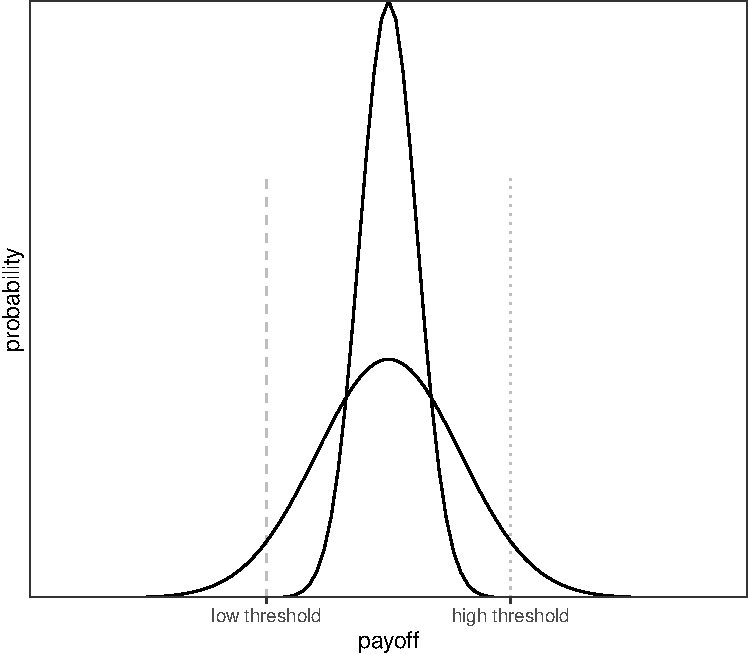
\includegraphics{rr-risk-sensitivity_files/figure-latex/varianceplot-1.pdf}
\caption{\label{fig:varianceplot}Survival thresholds. When fitness drops to zero below the low threshold (dashed line), individuals should be risk-averse because the outcomes of the low-risk option (narrow curve) are guaranteed to lie above the threshold and the outcomes of the high-risk option (wide cuve) have a non-negligible risk of falling below the threshold. When fitness drops to zero below the high threshold (dotted line), individuals should be risk-prone because only the high-risk option provides a chance of passing the threshold.}
\end{figure}

Although comparable cutoff points in academic careers may have somewhat less severe consequences, they certainly exist:
Amount and impact of a researcher's publications are common and often explicit criteria in decisions that are central to the individual's career, such as whether they will be awarded a PhD, whether they will receive grant funding, whether they will be offered a tenure-track position, or whether they will be granted tenure.
In some of these situations, the cutoff points are absolute and thus resemble survival thresholds in the biological sense, for example PhD-programme regulations that determine a minimal amount of peer-reviewed publications for a candidate to be awarded with a PhD, or tenure contracts that specify minimal publication targets.
In other situations, the cutoff points are relative and depend on the number of eligible candidates, for example when the 10 highest-ranked research proposals receive funding or the best candidate out of a pool of applicants is offered a job.
In cases like these, one individual's success diminishes the chances of other individuals\(\,\)---\(\,\)in other words, they represent \emph{competition}.
In the following, survival thresholds and competition will be treated as separate concepts to examine their differential effects on researchers' publication behaviour.

\hypertarget{number-of-decision-events-before-evaluation}{%
\paragraph{Number of decision events before evaluation}\label{number-of-decision-events-before-evaluation}}

A final factor with relevance to risk-sensitive behaviour considered in this chapter is the number of decision events taking place before an individual's fitness is evaluated.
When a risky option is chosen repeatedly, the average of the accumulating payoffs gets closer and closer to the long-run expected payoff.
This means that the danger of loosing out completely by only acquiring the lowest possible payoff of the risky option diminishes, making the risky option relatively more attractive.
However, this relationship only holds for repeated decision events \emph{before} an individual's fitness is evaluated.
When fitness is evaluated after each decision, choosing a risky option might yield an outcome that translates to zero fitness, meaning death or an ultimate failure to reproduce.
When one risky decision might cost an individual's life or offspring, average fitness is best described by the geometric mean instead of the arithmetic mean.
The geometric mean is more sensitive to variance because it is multiplicative, capturing the fact that one failure to reproduce can end a genetic lineage.
This circumstance has been shown to produce bet-hedging:
Risk-averse strategies may be more adaptive across many generations even when more risk-prone strategies produce better outcomes in any one generation, simply because the latter are also more likely to lead to extinction by sheer bad luck.
While average fitness across generations is best represented with the geometric mean, average fitness \emph{within} a generation is better captured by the arithmetic mean, reflecting the additive accumulation of payoffs from decision events before fitness is evaluated.
Therefore, as the number of decision events per generation (before fitness is evaluated) increases, the variance-sensitive geometric mean of acquired payoffs becomes relatively less important and the less variance-sensitive arithmetic mean becomes more important.
Consequently, individuals' behaviour should switch from relative risk aversion to relative risk-proneness.

In the academic system, decision events before fitness is evaluated (\enquote{per generation}) could seen as the time and resources a researcher has available for producing publications before a relevant decision like those mentioned in the previous section (award of a PhD or grant, job application, tenure decision) is made.
Regarding time, the number of publications PhD student or early-career researcher may be limited by
\textbf{NEEDS WORK}

Each of the factors described above\(\,\)---\(\,\)non-linear fitness functions, survival thresholds, competition, and the number of decision events prior to evaluation\(\,\)---\(\,\)likely impacts researchers' decison strategies, including their choices between low-risk and high-risk publication options.
To better understand when a low-risk option like Registered Reports should be particularly attractive or unattractive, I examine the individual and interactive effects of these factors in a simulation model.

\hypertarget{model-description}{%
\subsection{Model description}\label{model-description}}

We develop an evolutionary agent-based model which simulates a population of researchers who test hypotheses, (attempt to) publish the results either as Registered Reports or as standard reports, accumulate the payoffs for successful publications, and pass their publication strategies on to the next generation of researchers.

\hypertarget{research-phase}{%
\paragraph{Research phase}\label{research-phase}}

Consider a population of \(n = 200\) researchers.
Each researcher has a fixed publication strategy \(s\), called the submission threshold.
In each round of the research phase, researchers randomly pick a hypothesis to test in a study.
Hypotheses are true with prior probability \(p\), which is uniformly distributed between 0 and 1.
Before testing their chosen hypothesis, a researcher compares the prior \(p\) of their hypothesis with their submission threshold \(s\).
When \(p < s\), the researcher chooses to play it safe and test the hypothesis in a Registered Report.
When \(p \geq s\), the researcher chooses to gamble and test the hypothesis in a normal study which is then submitted as a stardard report.
For simplicity, we assume that \(p\) is an ideal objective prior and that researchers' hypothesis tests are free from additional sources of error.
Thus, when a researcher proceeds to testing hypothesis \(i\), they obtain a positive result with probability \(p_i\) and a negative result with probability \(1-p_i\).
If the researcher chose to conduct a Registered Report, their study gets published regardless of the result and the researcher receives a payoff \(b_{RR}\).
However, if the researcher chose to publish their results as a standard report, they face rampant publication bias:
Only positive results are publishable as standard reports and yield a payoff \(b_{SR+}\), whereas negative results are rejected or file-drawered and only yield a minimal payoff \(b_{SR-}\).
For all variations of the model tested here, we assume that \(b_{SR-} < b_{RR} < b_{SR+}\).
This assumption reflects the following considerations:

\begin{enumerate}
\def\labelenumi{\arabic{enumi}.}
\tightlist
\item
  Due to publication bias, negative results are less valuable than positive results (\(b_{SR-} < b_{SR+}\)), for example because they do not lead to a publication at all, because only very low-impact journals are willing to publish them, or because getting them published requires a lot of extra effort (e.g., via frequent resubmissions following rejection or substantial revisions demanded by reviewers) that diminishes the net reward.
\item
  These same reasons mean that Registered Reports are on average more valuable than standard reports with negative results (\(b_{SR-} < b_{RR}\)), for example because Registered Reports are offered by journals that may display publication bias and reject negative results in standard report submissions, or simply because Registered Reports do not need to be resubmitted or require more extensive revisions in case of a negative result.
\item
  On average, standard reports with positive results are more valuable than Registered Reports (\(b_{RR} < b_{SR+}\)), for example because most extremely high-impact journals (e.g., \emph{Science} and \emph{Nature}) do not (yet) offer Registered Reports, because not registering one's study \emph{a priori} makes it easier to spin the results into an attention-grabbing story, or because Registered Reports may require more effort due to their stricter quality criteria, lowering the net reward.
  While proponents of Registered Reports may argue that the format has such trememdous advantages that authors' resulting career benefits are superior to any alternative, this chapter is predicated on the fact that most researchers do not seem to share this view.
  Once this changes, the present investigation may happily become redundant.
\end{enumerate}

This research cycle\(\,\)---\(\,\)choosing a hypothesis, choosing a publication route by comparing its prior \(p\) to one's submission threshold \(s\), testing the hypothesis, and receiving payoff \(b_{RR}\) for a Registered Report or \(b_{SR-}\) or \(b_{SR+}\) for a positive and negative standard report, respectively\(\,\)---\(\,\)is repeated \(m\) times.

\hypertarget{evaluation-phase}{%
\paragraph{Evaluation phase}\label{evaluation-phase}}

At the end of the research phase, researchers are evaluated by translating their accumulated publication payoffs \(b_1 + b_2 + ... + b_m\) into fitness using exponent \(\epsilon\), which reflects the shape of the fitness function (\(\epsilon = 1\) yields a linear function, \(0 < \epsilon < 1\) yields a concave function with diminishing returns, \(\epsilon > 1\) yields a convex function with increasing returns, see Figure~\ref{fig:fitnessplot}):

\begin{align}
fitness = (\sum_{i=1}^{m} b_i)^\epsilon
\end{align}

However, two situations may cause a researcher's fitness to fall to zero even when their accumulated payoffs are nonzero.
First, the sum of their payoffs may fall below an absolute survival threshold \(\delta\), for example when a researcher fails to meet an agreed publication target by the time their \enquote{tenure clock} runs out.
Thus, when \(\sum_{i=1}^{m} b_i < \delta\), \(fitness = 0\).
Second, the sum of their payoffs may fall below a relative threshold \(\gamma\), which reflects the intensity of competition for scarce resources such as research grants or positions.
\(\gamma\) is the proportion of the most productive researchers that are considered for reproduction.
When \(\gamma = 1\), all researchers in the population are considered for reproduction and their fitness is calculated according to Eq. 1.
When \(\gamma < 1\), the \((1 - \gamma)\) portion of researchers with the lowest sum of payoffs receives zero fitness and cannot reproduce.\footnote{The computer code of the simulation applies \(\gamma\) after fitness has been calculated according to the accumulated payoffs. This change has purely technical reasons and yields the same result as calculating fitness after \(\gamma\) has been applied to accumulated payoffs, since all fitness functions are monotonic increasing.}
For example, \(\gamma = 0.1\) means that only those researchers with accumulated payoffs in the top \(10\%\) of the population can reproduce, and the remaining \(90\%\) receives zero fitness.

\hypertarget{reproduction-phase}{%
\paragraph{Reproduction phase}\label{reproduction-phase}}

Finally, the researchers in the current population retire and a new (non-overlapping) generation of researchers is created.
A researcher in the new generation inherits their publication strategy (submission threshold) \(s\) from a researcher in the previous generation with the probability of the previous researcher's fitness (i.e., the new generation's submission thresholds are sampled with replacement from the previous generation, probability-weighted by fitness).
The new generation's submission thresholds are inherited with a small amount of random noise, such that \(s_{new} = s_{old} + w\) with \(w \sim R(\mu = 0, \sigma = 0.01)\).
This evolutionary dynamic of researchers passing on their traits to other researchers depending on their career success can be seen as reflecting mentorship and explicit teaching, such as when established professors advise their students to use the same strategies, or simply a generic social learning process in which successful researchers are more likely to be imitated by others.

\hypertarget{outcome-variables}{%
\subsubsection{Outcome variables}\label{outcome-variables}}

We study how the evolution of researchers' submission thresholds \(s\) is affected by the payoff parameters \(b_{RR}\), \(b_{SR-}\), and \(b_{SR+}\), by the shape of the fitness function determined by exponent \(\epsilon\), by the absolute survival threshold \(\delta\), by competition \(\gamma\), and by the number of research cycles per generation \(m\) (see Table 1 for an overview of the model parameters and their values considered in the simulation).
It is important to keep in mind that a researcher's submission threshold \(s\) is a \emph{strategy}, not an absolute decision\(\,\)---\(\,\)it determines \emph{how} the choice between Registered Reports and standard reports is made, not which format is chosen.
As such, \(s\) indicates the amount of risk a researcher is willing to take.
Very low values of \(s\) reflect risk proneness:
The researcher is willing to gamble and chooses the standard publication route for almost all hypotheses they encounter, using the Registered Reports route only for hypotheses that are virtually guaranteed to be false (and yield negative results).
Very high values of \(s\) reflect risk aversion:
The researcher is unwilling to risk a negative result in a standard report and studies almost all hypotheses they encounter in the Registered Reports format, reserving the standard publication route only for hypotheses that are virtually guaranteed to be true (and yield positive results).

The evolved values of \(s\) over many generations indicate the optimal strategy for a given set of parameter values.

\hypertarget{results}{%
\section{Results}\label{results}}

When interpreting the results below, it is important to keep in mind that the analysed parameter values are arbitrary.
Although the model parameters are chosen to capture important characteristics of real-world concepts, the parameter values do not represent real-world units.
The goal of this analysis is to understand the general effects of the model parameters in an artificial world, meaning that the results are inherently relative.

The general principle of the simulation is shown in Figure~\ref{fig:evoplot}.



\begin{figure}
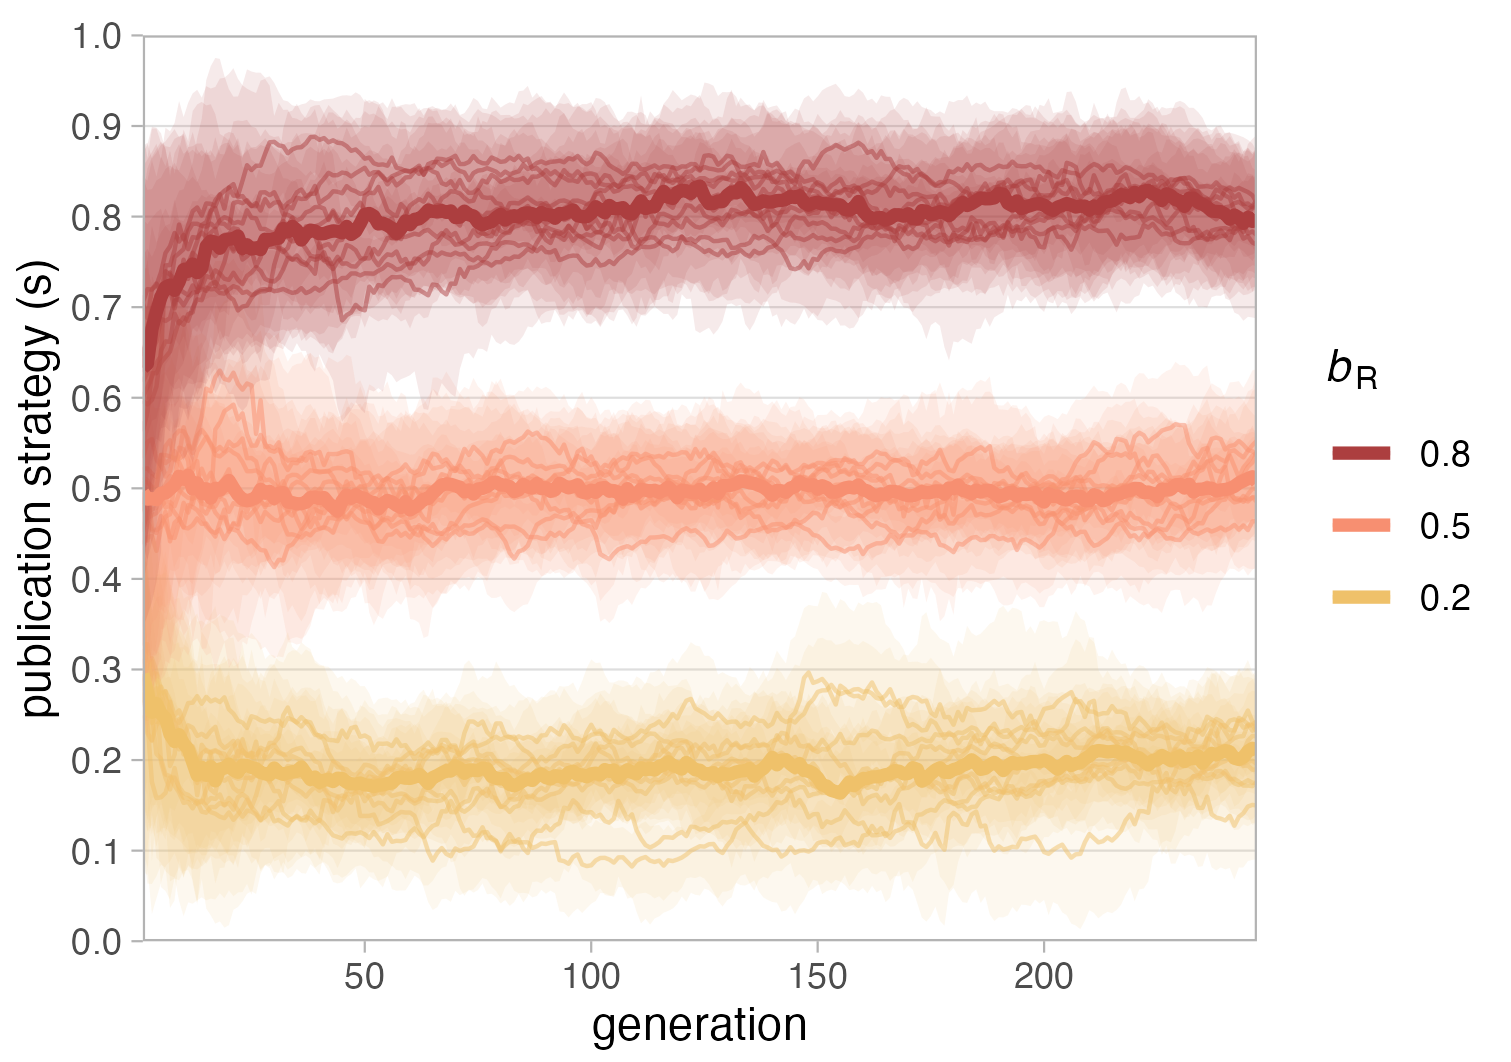
\includegraphics[width=5.04in]{/zephyr/Documents/Uni/_projects/rr-model/plots/plot_evo} \caption{Evolution of submission threshold for different values of \(b_{RR}\). Shown are 10 runs per condition over 250 generations. Thin lines represent the median submission threshold of the population in each run, shaded areas represent the inter-quartile range of submission thresholds in the population in each run, thick lines represent the median of run medians per condition.}\label{fig:evoplot}
\end{figure}

\hypertarget{non-linear-fitness-functions-1}{%
\subsection{Non-linear fitness functions}\label{non-linear-fitness-functions-1}}

A reference to Figure~\ref{fig:epsilonplot}.



\begin{figure}
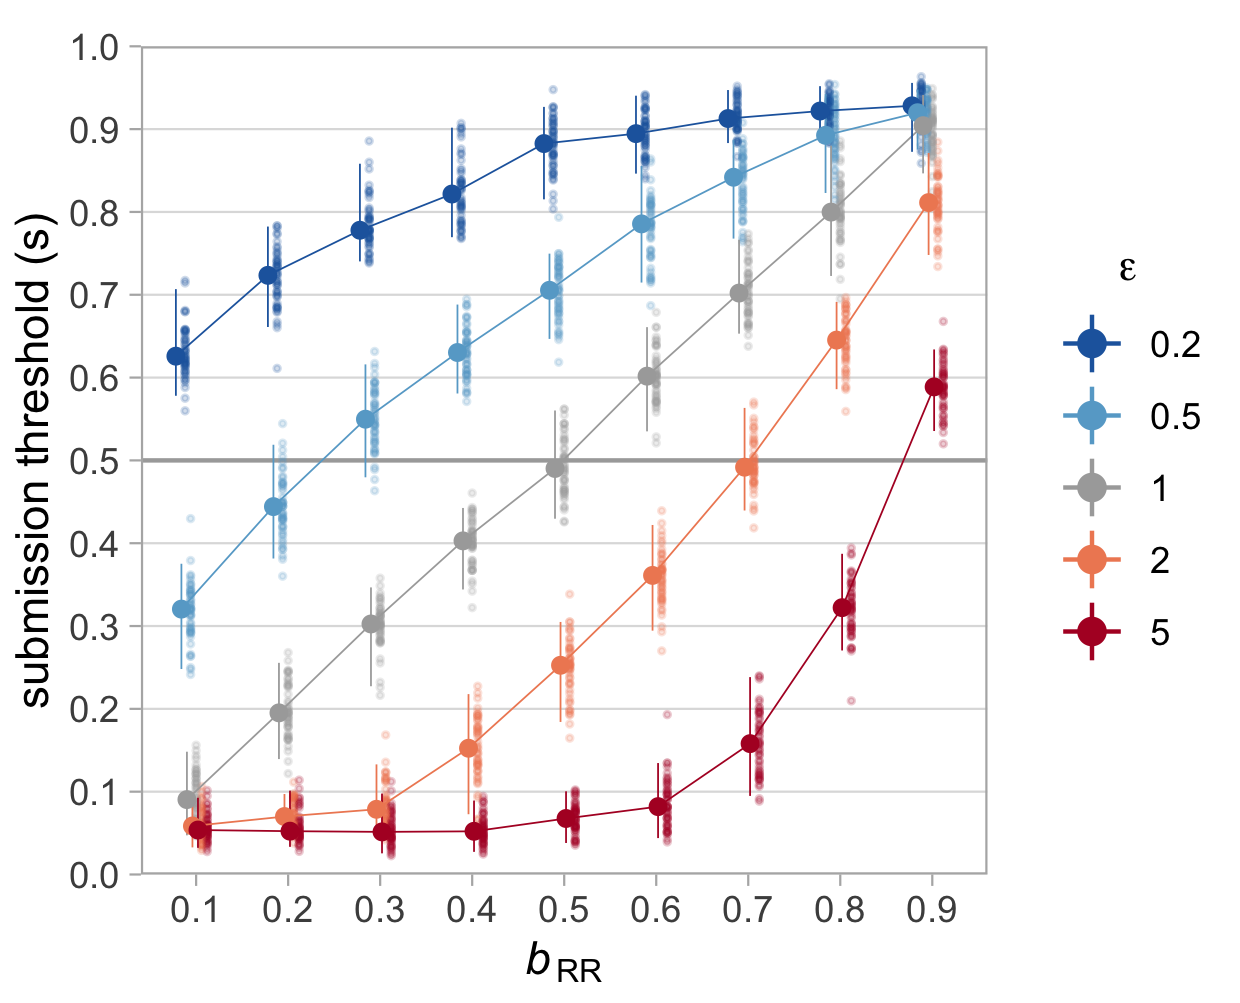
\includegraphics[width=0.65\linewidth]{/zephyr/Documents/Uni/_projects/rr-model/plots/plot_b_e} \caption{Figure note).}\label{fig:epsilonplot}
\end{figure}

\hypertarget{number-of-decision-events-before-evaluation-1}{%
\subsection{Number of decision events before evaluation}\label{number-of-decision-events-before-evaluation-1}}

A reference to Figure~\ref{fig:mplot}.



\begin{figure}
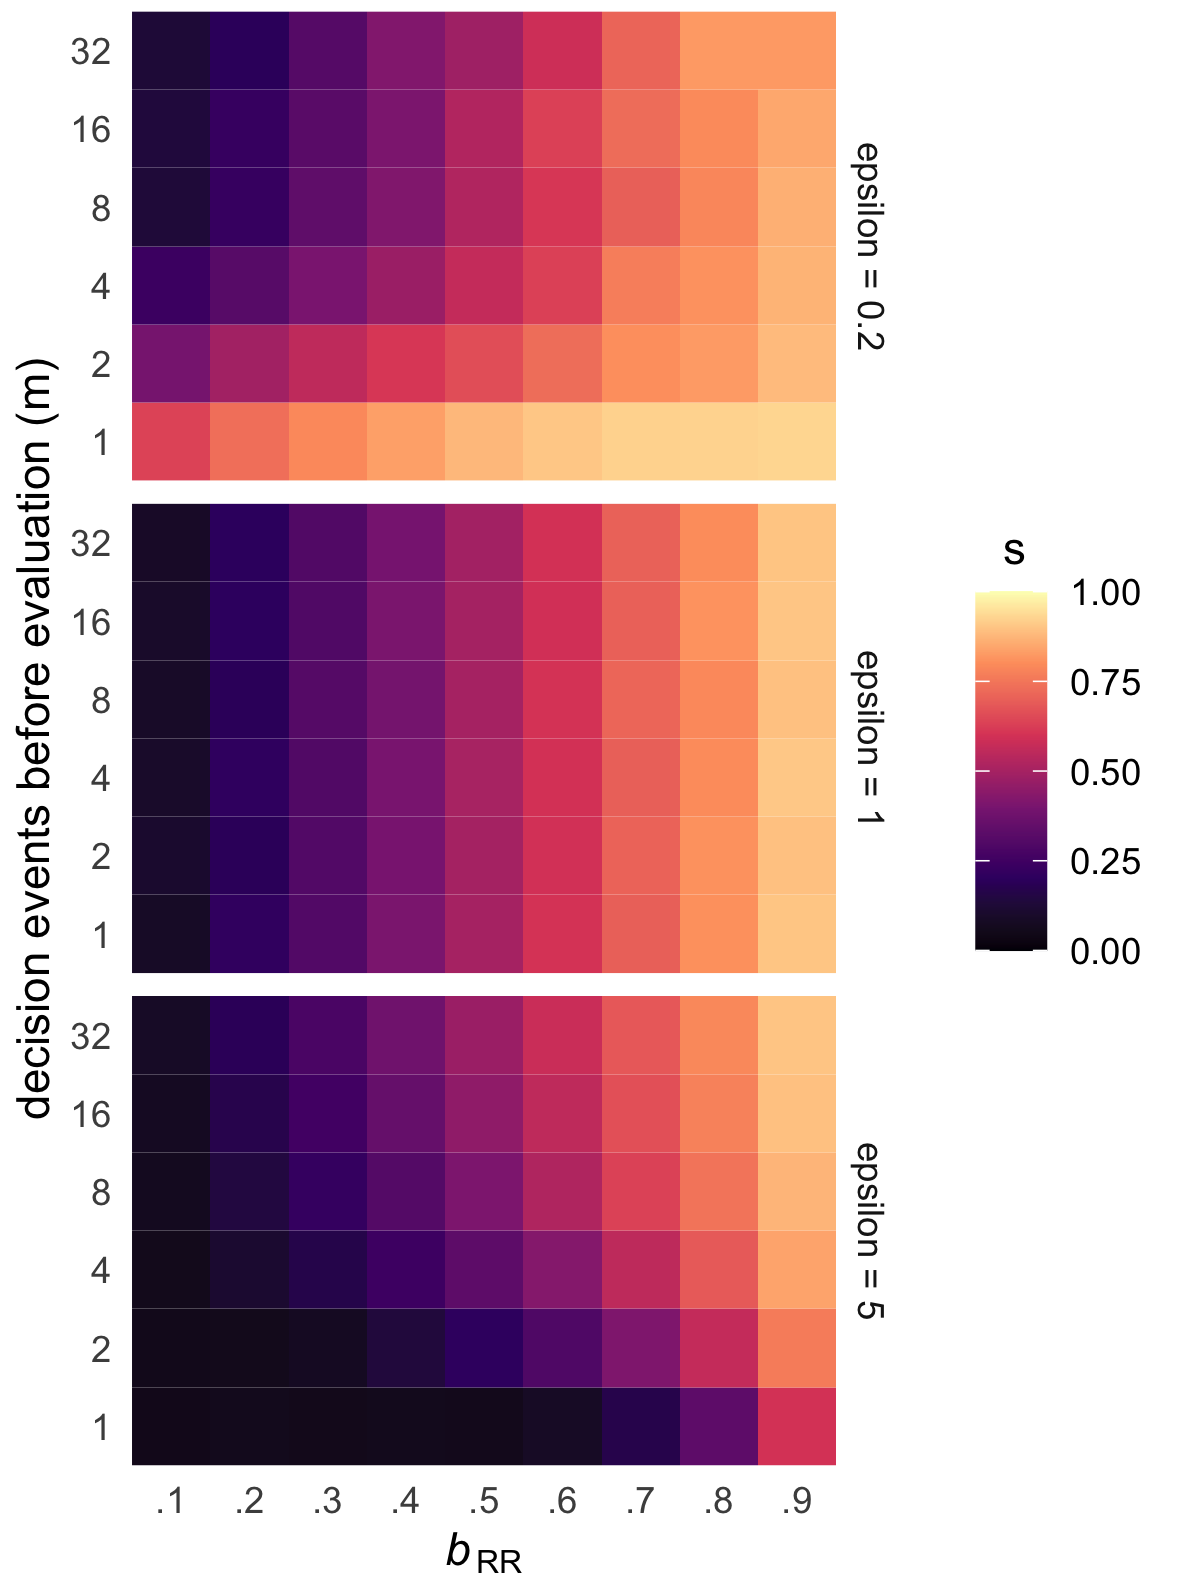
\includegraphics[width=0.5\linewidth]{/zephyr/Documents/Uni/_projects/rr-model/plots/plot_m} \caption{Figure note).}\label{fig:mplot}
\end{figure}

\hypertarget{survival-thresholds}{%
\subsection{Survival thresholds}\label{survival-thresholds}}

\hypertarget{competition}{%
\subsection{Competition}\label{competition}}

A reference to Figure~\ref{fig:competitionplot}.



\begin{figure}
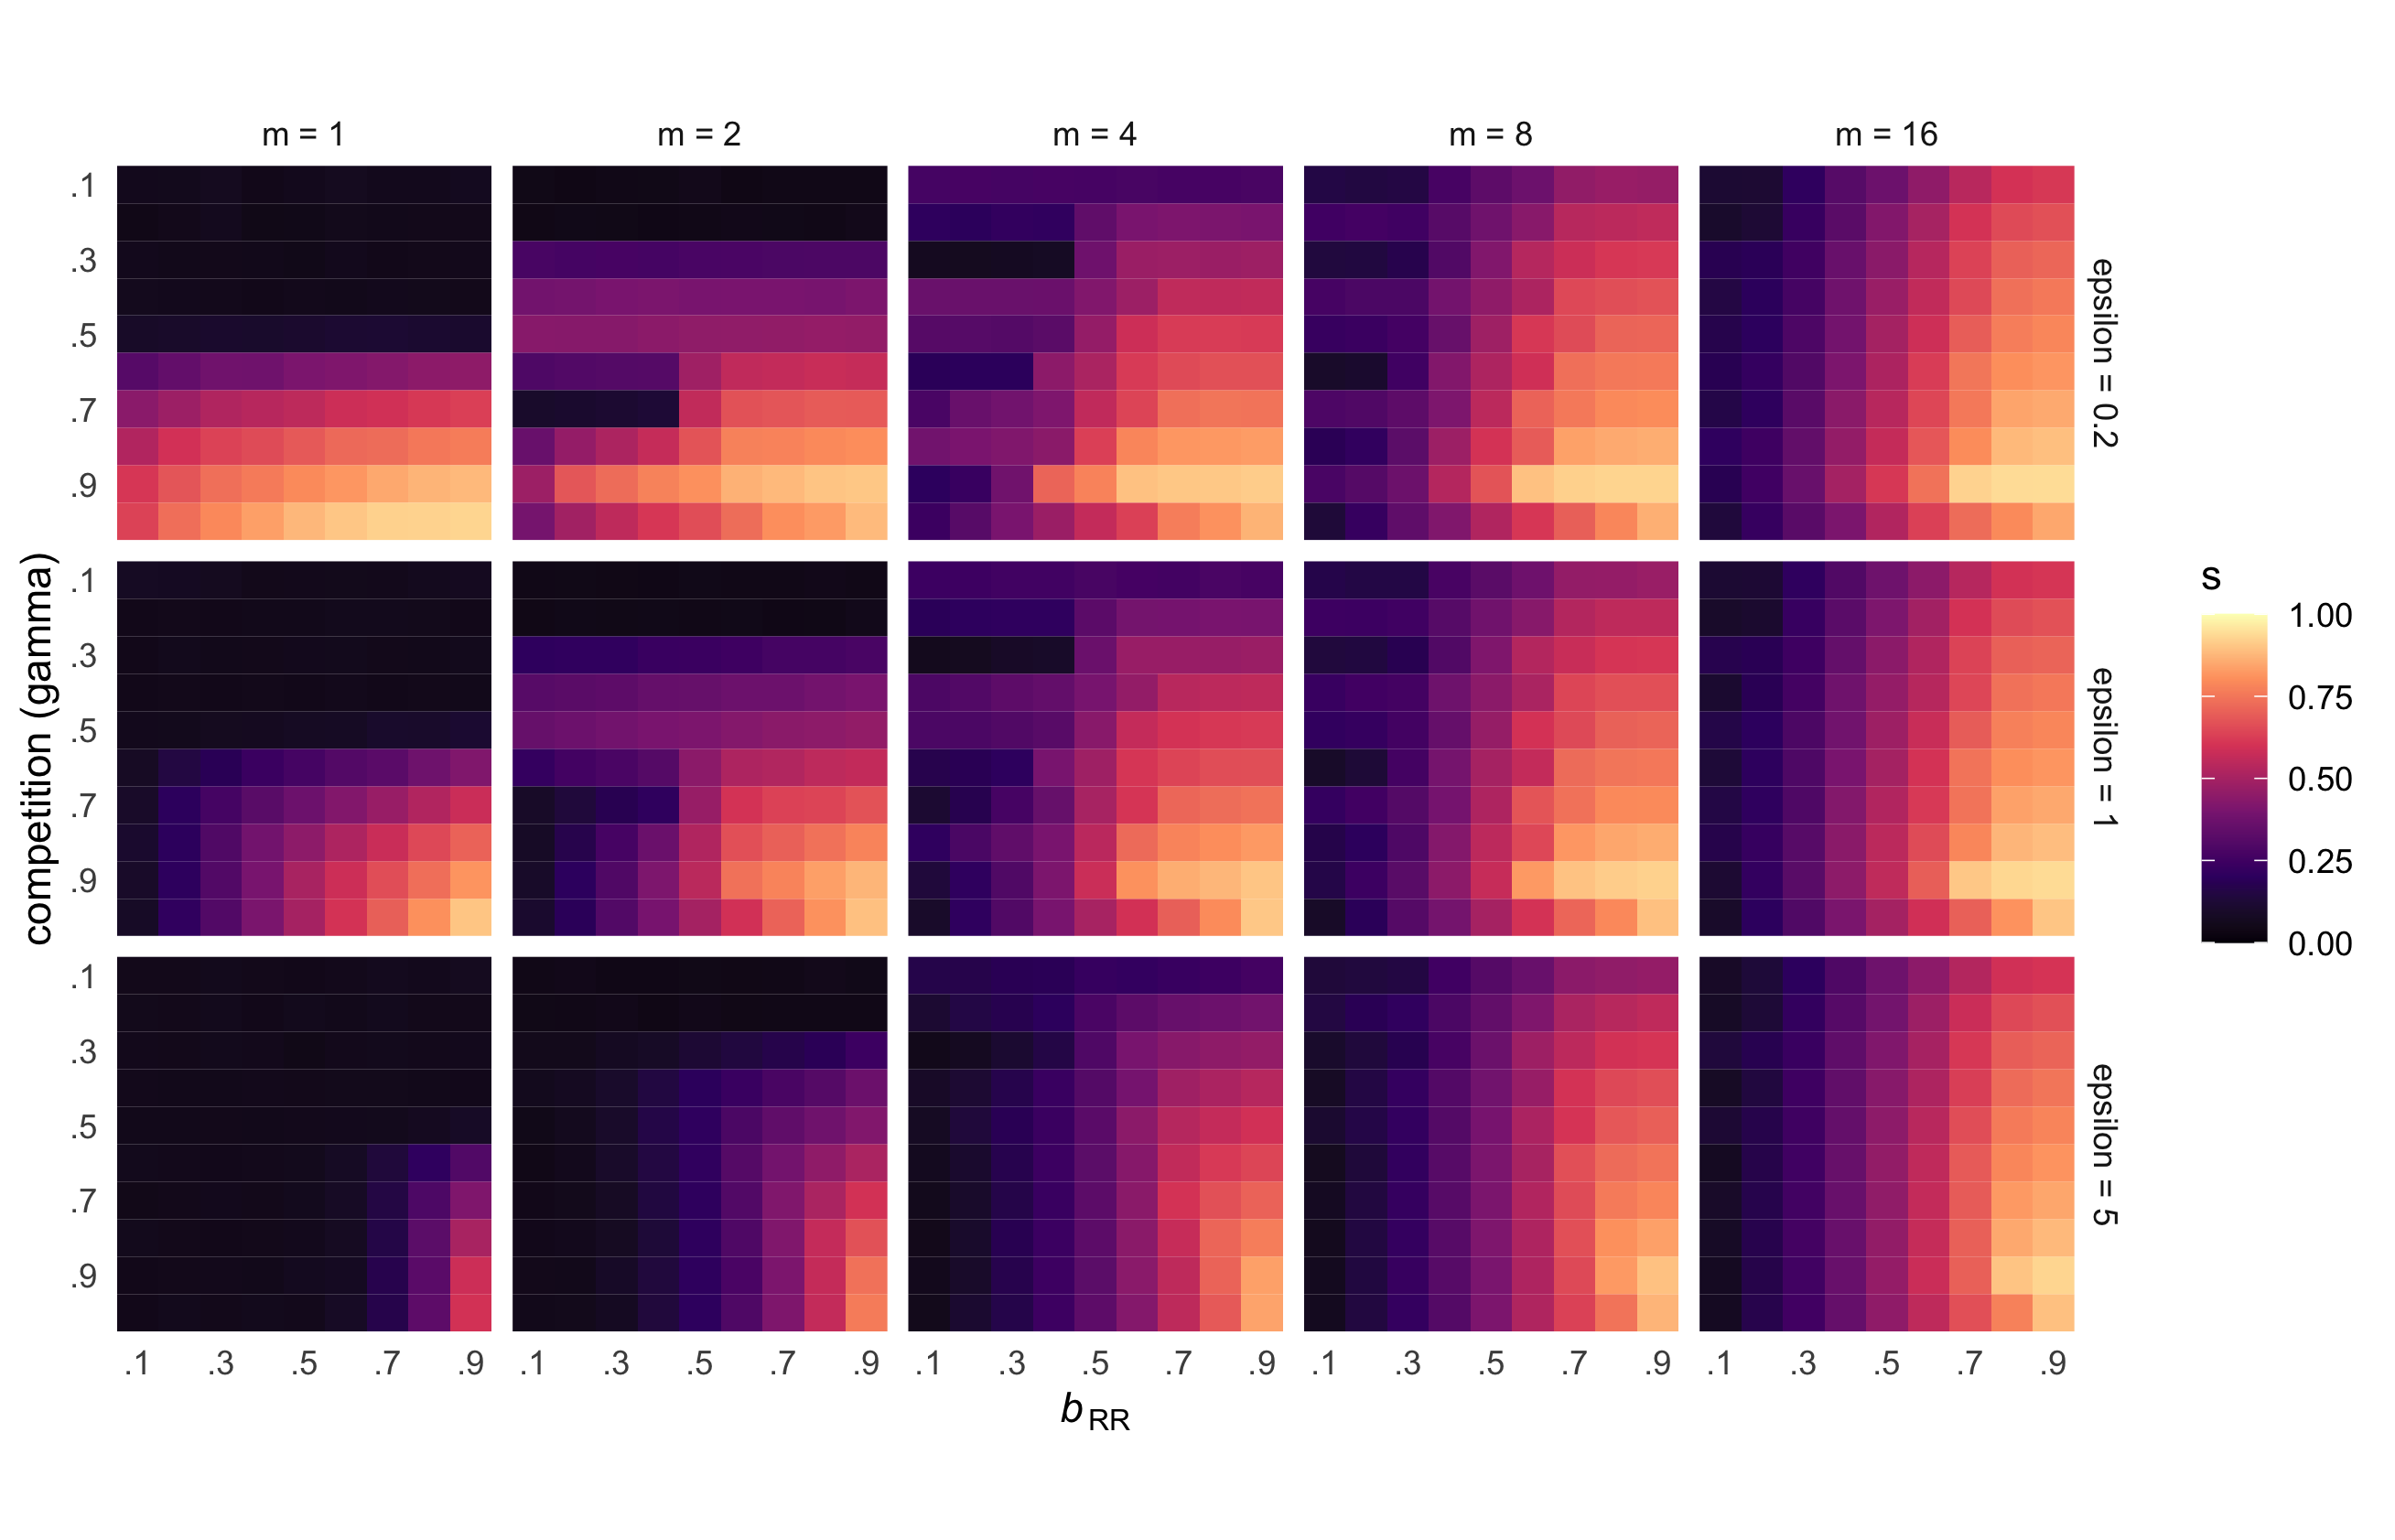
\includegraphics[width=1\linewidth]{/zephyr/Documents/Uni/_projects/rr-model/plots/plot_comp} \caption{Figure note).}\label{fig:competitionplot}
\end{figure}

\hypertarget{measures-and-coding-procedure}{%
\subsection{Measures and coding procedure}\label{measures-and-coding-procedure}}

Print settings from the script \enquote{utilitycurves\_plot.R}:

payoff\_RR is \(0.60\) and e\_low is 0.25.

\hypertarget{results-1}{%
\section{Results}\label{results-1}}

\hypertarget{discussion}{%
\section{Discussion}\label{discussion}}

\hypertarget{limitations}{%
\subsection{Limitations}\label{limitations}}

\hypertarget{future-directions}{%
\subsection{Future directions}\label{future-directions}}

\begin{itemize}
\tightlist
\item
  state-dependent risk taking (Barclay et al.): some researchers are more willing or able to tweak their results than others, making SRs more attractive(?)
\end{itemize}

\hypertarget{conclusion}{%
\subsection{Conclusion}\label{conclusion}}

\hypertarget{disclosures}{%
\subsection{Disclosures}\label{disclosures}}

\hypertarget{data-materials-and-online-resources}{%
\subsubsection{Data, materials, and online resources}\label{data-materials-and-online-resources}}

\href{https://osf.io/aqr2s/}{Data} and code necessary to reproduce all analyses reported here, as well as the \href{https://osf.io/qw798/}{Appendix}, the \href{https://osf.io/sy927/}{preregistration}, and additional supplementary files, are available at \url{https://osf.io/dbhgr}.
The manuscript, including figures and statistical analyses, the \href{https://osf.io/qw798/}{Appendix}, and the \href{https://osf.io/6jrkz/}{codebook} available in the supplement were created using RStudio (1.2.5019, {\textbf{???}}) and R (Version 3.6.0; R Core Team, 2019) and the R-packages \emph{bookdown} (Version 0.24; Xie, 2016), \emph{ggplot2} (Version 3.3.5; Wickham, 2016), \emph{here} (Version 1.0.1; Müller, 2020), \emph{knitr} (Version 1.37; Xie, 2015), \emph{papaja} (Version 0.1.0.9997; Aust \& Barth, 2018), \emph{rmarkdown} (Version 2.12; Xie, Allaire, \& Grolemund, 2018), \emph{stringr} (Version 1.4.0; Wickham, 2019), and \emph{tinylabels} (Version 0.2.3; Barth, 2022).

\hypertarget{reporting}{%
\subsubsection{Reporting}\label{reporting}}

We report how we determined our sample size, all data exclusions, all manipulations, and all measures in the study.

\hypertarget{author-contributions}{%
\subsubsection{Author Contributions}\label{author-contributions}}

Conceptualisation: A.S. \& D.L.; data curation, formal analysis, and software: A.S. \& M.R.M.J.S.; investigation, methodology, and validation: A.S., M.R.M.J.S., \& D.L; supervision: A.S \& D.L.; visualisation and writing\(\,\)---\(\,\)original draft: A.S; writing\(\,\)---\(\,\)review and editing: A.S., M.R.M.J.S., \& D.L.

\hypertarget{conflicts-of-interest}{%
\subsubsection{Conflicts of Interest}\label{conflicts-of-interest}}

The authors declare that they have no conflicts of interest with respect to the authorship or the publication of this article.

\hypertarget{acknowledgements}{%
\subsubsection{Acknowledgements}\label{acknowledgements}}

This work was funded by VIDI grant 452-17-013. We thank Chris Chambers, Emma Henderson, Leo Tiokhin, Stuart Ritchie, and Simine Vazire for valuable comments that helped improve this manuscript.

\hypertarget{references}{%
\section{References}\label{references}}

\setlength{\parindent}{-0.2in}
\setlength{\leftskip}{0.2in}

\hypertarget{refs}{}
\leavevmode\hypertarget{ref-R-papaja}{}%
Aust, F., \& Barth, M. (2018). \emph{papaja: Create APA manuscripts with R Markdown}.

\leavevmode\hypertarget{ref-R-tinylabels}{}%
Barth, M. (2022). \emph{tinylabels: Lightweight variable labels}. Retrieved from \url{https://cran.r-project.org/package=tinylabels}

\leavevmode\hypertarget{ref-R-here}{}%
Müller, K. (2020). \emph{Here: A simpler way to find your files}. Retrieved from \url{https://CRAN.R-project.org/package=here}

\leavevmode\hypertarget{ref-R-base}{}%
R Core Team. (2019). \emph{R: A language and environment for statistical computing}. Vienna, Austria: R Foundation for Statistical Computing.

\leavevmode\hypertarget{ref-Smaldino2016}{}%
Smaldino, P. E., \& McElreath, R. (2016). The natural selection of bad science. \emph{Royal Society Open Science}, \emph{3}, 160384. \url{https://doi.org/10.1098/rsos.160384}

\leavevmode\hypertarget{ref-R-ggplot2}{}%
Wickham, H. (2016). \emph{Ggplot2: Elegant graphics for data analysis}. Springer-Verlag New York.

\leavevmode\hypertarget{ref-R-stringr}{}%
Wickham, H. (2019). \emph{Stringr: Simple, consistent wrappers for common string operations}. Retrieved from \url{https://CRAN.R-project.org/package=stringr}

\leavevmode\hypertarget{ref-Winterhalder1999}{}%
Winterhalder, B., Lu, F., \& Tucker, B. (1999). Risk-senstive adaptive tactics: Models and evidence from subsistence studies in biology and anthropology. \emph{Journal of Archaeological Research}, \emph{7}(4), 301--348. \url{https://doi.org/10.1007/BF02446047}

\leavevmode\hypertarget{ref-R-knitr}{}%
Xie, Y. (2015). \emph{Dynamic documents with R and knitr} (Second). Boca Raton, Florida: Chapman and Hall/CRC.

\leavevmode\hypertarget{ref-R-bookdown}{}%
Xie, Y. (2016). \emph{Bookdown: Authoring books and technical documents with R markdown}. Boca Raton, Florida: Chapman and Hall/CRC.

\leavevmode\hypertarget{ref-R-rmarkdown}{}%
Xie, Y., Allaire, J., \& Grolemund, G. (2018). \emph{R markdown: The definitive guide}. Boca Raton, Florida: Chapman and Hall/CRC.


\end{document}
